%%
%% This is the documentation of `matapli.cls',
%%
%% -----------------------------------------------------------------------------
%% MATAPLI --- SMAI bundle of classes for the French journal "MATAPLI",
%% version 1.0.0
%%
%% author : Maxime Chupin
%% E-mail: chupin@ceremade.dauphine.fr
%% Released under the LaTeX Project Public License v1.3 or later
%% See http://www.latex-project.org/lppl.txt
%% -----------------------------------------------------------------------------

\documentclass{mataplidoc}

\usepackage{multicol}
\usepackage{pdfpages}

\title{Classe \Verb+matapli+ pour la revue MATAPLI de la SMAI}
\author{Maxime \bsc{Chupin} \email{chupin@ceremade.dauphine.fr}}
\date{\today}

\addbibresource{bibliomatapli.bib}

\begin{document}
%% === Page de garde ===================================================
\thispagestyle{empty}
\begin{tikzpicture}[remember picture, overlay]
  \node[below right, shift={(-4pt,4pt)}] at (current page.north west) {%
    
\includegraphics{fond-doc.pdf}%
  };
\end{tikzpicture}%

\noindent

\includegraphics{matapli-title}\\
{\large Documentation de la classe MATAPLI pour la revue de la SMAI}\\[1cm]
\vspace{2cm}

\hfill\parbox{0.3\textwidth}{\Large\raggedleft
  \textbf{Contributor}\\
  Maxime \textsc{Chupin}
}
\vfill
\begin{center}
  Version 1.1, 22 mars 2021 \\
  \url{https://plmlab.math.cnrs.fr/mchupin/matapli}
\end{center}
%% == Page de garde ====================================================
\newpage

\maketitle

\begin{abstract}
  La classe \LaTeX{} \Verb+matapli+ est destinée à la composition de la revue
  MATAPLI de la SMAI. Cette classe  contient à la fois les éléments
  permettant de rédiger un article pour cette revue et les éléments
  permettant de composer la revue dans sa globalité.
\end{abstract}

\begin{center}
  \url{https://plmlab.math.cnrs.fr/mchupin/matapli}
\end{center}


\tableofcontents
\bigskip

\noindent\textbf{Avertissement :} Les exemples présentés dans cette
documentation ne sont malheureusement pas accompagnés du rendu après
compilation. Pour voir ce que produisent ces exemples, il faudra aller
voir les documents d'exemples fournis (voir section~\ref{sec:exemples}).

\noindent\textbf{Remerciement :} Je tiens à remercier Denis \bsc{Bitouzé} pour
ses conseils, et ses productions, avec en particulier~\cite{gazette,yathesis},
qui sont sources d'inspiration.

\section{Installation}

La classe \matapli{} est disponible sur le CTAN pour toute installation
récente d'une distribution \LaTeX.

\begin{center}
  \url{https://www.ctan.org/pkg/matapli}
\end{center}

Vous pouvez évidemment aussi utiliser le fichier \Verb+matapli.cls+
dans votre répertoire de travail.


\subsection{Avec \TeX live sous linux et Mac OSX}

Pour installer la classe \matapli{} avec \TeX live, il vous faudra
créer, si ce n'est déjà fait, un répertoire local \Verb+texmf+ dans
votre \Verb+home+ pour ensuite y placer le fichier \Verb+matapli.cls+
en créant l'arborescence nécessaire, dans le répertoire :
\begin{center}
  \Verb+~/texmf/tex/latex/matapli/+
\end{center}
Une fois cela fait, vous pourrez charger la classe \matapli{}
simplement avec le classique :
\begin{latexcode}
  \documentclass{matapli}
\end{latexcode}

\subsection{Avec Mik\TeX{} et Windows}

Ces deux systèmes sont inconnus du mainteneur de la classe \matapli{}
aussi nous renvoyons à la documentation :
\begin{center}
  \url{http://docs.miktex.org/manual/localadditions.html}
\end{center}

\section{Utilisation}

Comme toute classe, \matapli{} se charge avec la commande
\Verb+\documentclass+. Comme cette classe est conçue pour être
utilisée avec \texttt{pdflatex} ou \texttt{lualatex}, si
\texttt{pdflatex} est utilisé, il ne faudra pas oublié de renseigner
l'encodage utilisé.

\begin{latexcode}
\documentclass{matapli}
%% si pdflatex
% \usepackage[utf8]{inputenc}

\begin{document}

\end{document}
\end{latexcode}

\subsection{Modèles d'utilisation}\label{sec:exemples}

Un modèle est  fourni avec la classe \matapli{}  dans le répertoire
\texttt{modeleauteur}, à destination des
auteurs et autrices qui écrivent pour la revue. Il est constitué d'un exemple
simple d'utilisation de la classe \matapli{} (à compiler avec
\texttt{pdflatex} mais peut être adapté à \texttt{lualatex}).

L'exemple fait un tour rapide des fonctionnalités offertes par la
classe \matapli{}.

\section{Pour les auteurs et autrices d'article}

Cette partie de la documentation concerne les auteurs ou autrices
désirant écrire un article pour la revue MATAPLI.

\subsection{Le titre de l'article}\label{sec:titre}

Le titre de l'article se renseigne avec la commande :

\commande|\titre[«options»]{«titre de l'article»}|\medskip

Cette commande offre deux options :
\begin{description}
\item[\Verb+court+ :] qui permet de renseigner un titre court pour le
  sommaire et les têtes de page.
  \begin{latexcode}
    \titre[court={Mon titre court}]{Mon titre plus long}
  \end{latexcode}
  \item[\Verb+auteur=article/partie+ :] qui permet de spécifier si les auteurs ou
    autrices sont relatives à l'article (chapitre) entier, ou aux
    sous-partie (voir section~\ref{sec:section}). La valeur par défaut
    est \Verb+article+. \emph{Noter que cette option est à ignorer par les
    contributeurs et contributrices à la revue MATAPLI.}
\end{description}


\subsection{Informations des auteurs et autrices}

Les auteurs et autrices d'une article (chapitre) ou d'une partie (voir
section suivante) sont à renseigner avec la commande \Verb+\author+
qui est redéfinie par rapport au comportement classique de \LaTeX. Il
faudra appeler cette commande pour chaque auteur ou autrice.

\commande|\author[«options»]{«Nom», «Prénom»}|\medskip

Les options sont sous forme de \texttt{clé=valeur} séparées par des
virgules. Voici la liste de ces options :

\begin{description}
\item[\Verb+affiliation=\{\meta{Laboratoire, université, etc.}\}+ :
  ] qui permet d'indiquer l'affiliation de l'auteur ou de l'autrice,
  c'est-à-dire, son laboratoire, son université, son organisme de
  recherche, son entreprise, etc. On veillera à mettre des accolades
  autour de l'affiliation.
\item[\Verb+email=\meta{email}+ : ] qui permet d'indiquer l'email
  de l'auteur ou autrice. On veillera à mettre l'email en texte brut,
  c'est-à-dire à \emph{ne pas mettre de commandes pour formater
    l'adresse} du type de \verb+\url+ ou \verb+\texttt+.
\item[\Verb+minibio=\{\meta{Petite biographie de l'auteur}\}+ : ] qui
  permet d'indiquer une bibliographie courte  qui est composée dans
  l'encart généré en fin d'article (voir section~\ref{sec:encart}).
\item[\Vert+photo=\meta{nomdufichierimage}+ : ] qui permet d'afficher
  une photo dans l'encart généré en fin d'article (voir
  section~\ref{sec:encart}). Il faut indiquer le nom du fichier (qui
  sera chargé par un \Verb+\includegraphics+), avec s'il a lieu, le
  chemin pour y accéder.
\item[\Verb+webpage=\meta{url de la page web}+ : ] qui permet de
  renseigner l'url d'une page web relative à l'auteur ou autrice qui
  sera composé dans l'encart généré en fin d'article (voir
  section~\ref{sec:encart}).
\item[\Verb+type=\meta{unique ou collectif}+ : ] qui permet de
  spécifier le type d'auteur pour permettre de renseigner un collectif
  (qui ne suit pas la structure nom, prénom). Les deux valeurs
  possibles sont \Verb+unique+ ou \Verb+collectif+ et la valeur par
  défaut est \Verb+unique+.
\end{description}

On pourra utiliser les options comme l'exemple suivant le montre.
\begin{latexcode}
  \author[
  affiliation = {CNRS, Université de Paris},
  minibio = {Paul \bsc{Lefevre} est Ingénieur de Recherche au CNRS
    affecté à l'université de Paris. Ses spécialités sont nombreuses.},
  photo = portrait.jpg,
  email = lefrevre@universite.fr,
  webpage = www.paul.com
  ]
  {Lefevre,Paul}

\author[type=collectif,
webpage = www.cnrs.fr,
photo = logoCNRS.fr
]{Centre National de la Recherche Scientifique}
\end{latexcode}

\subsection{Commande pour générer l'affichage des auteurs et
  autrices. }\label{sec:printauthors} Les commandes de définition d'auteurs et d'autrices se
couplent avec l'utilisation de la commande

\commande|\printauthors[«option»]|\medskip

Cette commande se place à la fin de l'article (du chapitre), ou de la
partie.

La seule option possible est destinée aux articles (au chapitres) où
les auteurs et autrices sont définies pour \emph{les parties} (et non
pour l'entièreté de l'article). Pour cela il faudra utilise l'option
\Verb+partie+ couplée à l'option similaire pour la commande
\Verb+\partie+ (voir section~\ref{sec:section}).

\begin{latexcode}
  \printauthors[partie]
\end{latexcode}

Le mécanisme de gestion des auteurs et autrices repose sur la création
de fichiers auxiliaires. Ainsi, il faudra compiler le document
\emph{deux fois} pour obtenir le résultat final.

\subsubsection{Encart généré}\label{sec:encart}

À la suite de la commande \Verb+\titre+ (ou \Verb+\partie+), les
auteurs et autrices sont indiqué·e·s avec leur noms et prénoms,
l'affiliation et, en note de pied de page, leur adresse email si
celle-ci est renseignée.

Si les biographies courtes des auteurs ou des autrices sont
renseignées dans les commandes \Verb+\author+, alors des encarts avec
les différentes informations des auteurs et autrices seront générés à
l'endroit de la commande \Verb+\printauthors+.


\subsection{Le sectionnement de l'article}\label{sec:section}

Le sectionnement de l'article est un sectionnement classique de
\LaTeX{} avec la classe \Verb+book+. Un article de MATAPLI est en fait
un chapitre d'une classe \Verb+book+ au détail prêt qu'il a été
rajouté la commande

\commande|\partie[«option »]|\medskip

Celle-ci permet de créer des parties à l'intérieur d'un article
(chapitre), et est donc \emph{au dessus} des \Verb+\section+. Les
compteurs des \Verb+(sub*)section+ sont mis à zéro à chaque partie.

\begin{latexcode}
\titre[Mon titre court]{Le titre long}

\partie{Une partie}
\section{Une section}
\subsection{Sous-section}
\subsubsection{Sous-sous-section}
\partie{Deuxième partie}
\section{Une section}
\end{latexcode}

La seule option possible est la suivante :
\begin{description}
\item[\Verb+auteur=\{\meta{article,partie}\}+ : ] par défaut, la valeur est à
  \Verb+article+, lors que les auteurs ou autrices sont renseigné pour l'article
  (le chapitre) entier. Si on souhaite avoir des auteurs ou autrices pour
  chacune des sous parties, alors, conjointement à la même option pour la
  commande\Verb+\titre+, il faudra mettre l'option \Verb+auteur=partie+. Dans ce
  cas, il faudra utiliser l'option \Verb+partie+ pour la commande
  \Verb+\printauthors+ (section~\ref{sec:printauthors}).
\end{description}

\subsection{Quelques commandes et environnements spécifiques}

La classe \matapli{} fournit quelque commandes et environnements
propres à la classe.

\subsubsection{Les packages chargés par la classe}

La classe \matapli{} fournit toutes les commandes des packages
suivants (chargés par la classe\footnote{Nous ne listons ici que les
  packages fournissant des commandes du côté utilisateur, et non tous
  les package chargés par la classe \matapli{}.}):
\begin{multicols}{2}
  \begin{itemize}
  \item la classe \Verb+book+ ;
  \item \Verb+latexsymb+, \Verb+amssymb+, \Verb+amsthm+,
    \Verb+mathtools+ ;
  \item \Verb+subfig+ ;
  \item \Verb+FiraSans+ et \Verb+newtxsf+ ;
  \item \Verb+babel+ avec les options \Verb+english,french+ ;
  \item \Verb+adjustbox+ ;
  \item \Verb+enumitem+ ;
  \item \Verb+graphicx+ ;
  \item \Verb+xcolor+ ;
  \item \Verb+fancyhdr+ et \Verb+fancybox+ ;
  \item \Verb+multicol+ ;
  \item \Verb+tabularx+ et \Verb+booktabs+ ;
  \item \Verb+url+ et \Verb+hyperref+ ;
  \item \Verb+tikz+ et \Verb+tcolorbox+ ;
  \item \Verb+biblatex+.
  \end{itemize}
\end{multicols}

\subsubsection{Quelques encadrés}

La classe \matapli{} fournit deux environnements permettant de mettre en relief
du contenu.

\commande|\begin{bloc}|

\commande|\end{bloc}|\medskip

et


\commande|\begin{Important}|

\commande|\end{Important}|\medskip

Pour voir ce que produisent ces environnement, nous renvoyons à la section~\ref{sec:exemples}.

\subsubsection{Pour les mathématiques}

Nous fournissons quelques environnements pour la composition des
mathématiques. Pour les définitions et les théorèmes, nous utilisons
le package \Verb+tcolorbox+, ce qui fait que les environnements dédiés
nécessitent un deuxième argument qui permet de renseigner un
\Verb+label+.

\paragraph{L'environnement \texttt{theorem}. } L'environnement pour les
théorèmes est le suivant :

\commande|\begin{theorem}{«Titre du théorème»}{«label»}|

\commande|\end{theorem}|\medskip

Les titres et labels peuvent être laissés vides. Notez que le label à
appeler lors de la référence au théorème est à préfixé de \Verb+th:+
comme l'illustre le code suivant :
\begin{latexcode}
  \begin{theorem}{Test}{test}
    Voici mon Théorème, classique, mais efficace.
  \end{theorem}

  \begin{proof}
    On y fait référence~\ref{th:test} pour en écrire la preuve.
  \end{proof}
\end{latexcode}

\paragraph{L'environnement \texttt{definition}. }
L'environnement pour les définitions suit la même syntaxe que celui
pour les théorèmes.

\commande|\begin{definition}{«Titre de la définition»}{«label»}|
\commande|\end{definition}|\medskip

\paragraph{Autres environnements classiques. }
La classe \matapli{} fournit aussi des environnements plus classiques
(construit avec l'extension \Verb+ntheorem+) que nous listons
ci-dessous. Ici, les environnements ne prennent pas de \emph{label} en
argument, il faudra donc les ajouter avec la commande \Verb+\label{}+
le cas échéant.
\begin{description}
\item[L'environnement \Verb+lemma+ : ] pour la composition des lemmes.
  \begin{latexcode}
    \begin{lemma}
      Un petit lemme.
    \end{lemma}
  \end{latexcode}
\item[L'environnement \Verb+corollary+ : ] pour la composition des
  corollaires.
  \begin{latexcode}
    \begin{corollary}
      Un corollaire.
    \end{corollary}
  \end{latexcode}
\item[L'environnement \Verb+remark+ : ] pour la composition des
  remarques.
  \begin{latexcode}
    \begin{remark}
      Une remarque.
    \end{remark}
  \end{latexcode}
\item[L'environnement \Verb+proof+ : ] pour la composition des
  preuve.
  \begin{latexcode}
    \begin{proof}
      Une preuve.
    \end{proofx}
  \end{latexcode}
\end{description}

\subsection{Gestion de la bibliographie}

La classe \matapli{} charge le package \Verb+biblatex+~\cite{biblatex}
pour la gestion bibliographique avec le moteur~\texttt{biber}. Il faudra
donc vous plier à ce fonctionnement. On pourra
consulter~\cite{BitouzeWeb} pour une introduction à \Verb+biblatex+
(et \LaTeX{} en général).

\subsubsection{Chargement du fichier de bibliographie}

Il faudra charger le fichier bibliographique \Verb+.bib+ avec la
commande suivante dans le préambule du document\footnote{Lors de la
  soumission d'article, essayer de fournir des noms de fichiers
  indiquant l'article en question, soit par une référence au titre, le
nom de l'auteur ou autrice, etc.}.
\begin{latexcode}
  \addbibresource{Monfichier.bib}
\end{latexcode}

\subsubsection{Imprimer la bibliographie}

Pour composer la liste des références bibliographiques on utilisera la
commande suivante à l'endroit où l'on souhaite la composer :
\begin{latexcode}
\printbibliography[heading=subbibintoc]
\end{latexcode}

Cette commande va afficher la liste des références en \emph{section}
(et non \emph{chapitre} comme le fonctionnement par défaut), et
l'ajoute à la table des matières.

\subsubsection{La compilation}

Il faudra suivre la procédure de compilation suivante, en supposant
que votre document \LaTeX{} est \texttt{mondocument.tex}:
\begin{enumerate}
\item \Verb+pdflatex+ ou \Verb+lualatex+ \texttt{mondocument.tex};
\item \Verb+biber+ \texttt{mondocument} (sans l'extension
  \texttt{.tex}) ;
\item \Verb+pdflatex+ ou \Verb+lualatex+ \texttt{mondocument.tex};
\item \Verb+pdflatex+ ou \Verb+lualatex+ \texttt{mondocument.tex}.
\end{enumerate}

\subsection{Pour les articles \emph{interview}}

Pour les articles sous forme d'interview, la classe \matapli{} fournit
deux commandes. La première permet de composer les questions :

\commande|\MatapliQuestion[«Nom optionnel»]{«Une question posée»}|\medskip

L'argument optionnel permet de renseigner le nom de la personne posant
la question comme l'illustre l'exemple suivant :
\begin{latexcode}
  \MatapliQuestion[Frédérique Dupont]{Que se passe-t-il ?}

  \MatapliQuestion{Question sans nom pour la poser ?}
\end{latexcode}


La deuxième commande permet de composer les réponses.

\commande|\MatapliReponse{«Nom»}{«Réponse»}|\medskip

Ici le nom de la personne interviewée est à renseigner obligatoirement
en premier argument.
\begin{latexcode}
\MatapliReponse{Laurent Faitlepain}{Un courte réponse qui suffit largement.}
\end{latexcode}


\subsection{Table des matières pour l'article}

Il est possible de produire une table des matières locale, relative à
l'article (le chapitre) en cours. Cela se fait avec la commande de la
classe \matapli{} :
\commande|\articletableofcontents|\medskip

qu'il faudra placer juste après la commande \Verb+\titre+.

\section{Pour la production de la revue}

Dans cette partie, sont documentés les éléments qui servent plutôt à
la production des numéros complets de la revue.

\subsection{Gestion des auteurs par parties d'un même article}

La classe \matapli{} permet de renseigner des auteurs et autrices par
sous partie d'un même article (chapitre). Pour cela, il faudra:
\begin{itemize}
\item utiliser la commande \Verb+\titre+ avec l'argument \Verb+auteur=partie+
comme décrit en section~\ref{sec:titre} ;
\item utiliser les commandes \Verb+\parties+ avec l'argument
  \Verb+auteur=partie+ comme décrit en section~\ref{sec:section} ;
\item renseigner les auteurs et autrices après les commande de
  \Verb+\partie+ avec les commandes \Verb+\author+ décrites en
  section~\ref{sec:printauthors} ;
\item utiliser la commande \Verb+\printauthors+ à la fin de la partie
  avec l'option \Verb+partie+ comme décrit en section~\ref{sec:section}
  pour chaque partie.
\end{itemize}

\subsection{Faire apparaître les traits de coupe sur du A4}

Pour l'envoie à l'impression, il suffit de charger dans le préambule :
\begin{latexcode}
  \usepackage[cam,a4,center]{crop}
\end{latexcode}

\subsection{Le sommaire}

Pour générer le sommaire, il suffit d'utiliser la commande :

\commande|\sommaire|\medskip

qui est un simple \Verb+\tableofcontents+ avec une profondeur à zéro
et dont l'affichage est un peu modifié.


\subsection{Les correspondant·e·s}

Pour composer les correspondant·e·s de la SMAI dans les divers
laboratoires et centres de recherche, la classe \matapli{} fournit la
commande suivante :

\commande|\correspondant{«ville»}{«Nom  Prénom»}{«laboratoire/université»}{«email»}|\medskip

Voici un exemple :
\begin{latexcode}
\correspondant{Avignon}{Karime Laporte}{%
Dépt. de Mathématiques\\
Univ. d'Avignon\\
33 rue Louis Pasteur\\
84000 Avignon\\
}{karime@laporte.fr}
\end{latexcode}


\subsection{Les colloques}

Pour composer les entrées de colloques pour la rubrique dédiée de la
revue MATAPLI, la classe \matapli{} fournit la commande suivante :

\commande|\colloque{«Titre du colloque»}{«date et lieu»}{«site web»}|\medskip

Attention, il ne faut pas mettre le site web en argument de  la commande
\Verb+\url+.

Voici un exemple qui permet de fixer les idées :
\begin{latexcode}
  \colloque{Journées sur l'analyse statistique et la quantification de l'incertitude des modèles numériques complexes (GdR Mascot num)}
  {du 27 au 30 Avril 2021, à Aussois}
  {https://www.gdr-mascotnum.fr/mascot20.html}
\end{latexcode}

\subsection{Les soutenances de doctorat et d'HDR}

Pour composer les entrées de soutenance de thèse dans la rubrique
dédiée de la revue MATAPLI, la classe \matapli{} fournit deux
environnements.

\subsubsection{Pour les thèses doctorat}

Pour les thèses de doctorat, on utilisera l'environnement suivant
encapsulant la description de la thèse :

\commande|\begin{soutenance}{«nom du/de la docteure»}{«date et lieu»}{«titre»}{«nom du ou de la directrice»}|

\commande|\end{soutenance}|\medskip


Voici un exemple d'utilisation de cet environnement :

\begin{latexcode}
  \begin{soutenance{Dimitri BIENFAIT}%
      { Soutenue le 10 octobre 2020 \\ Laboratoire Louis Lagrange et
        Université de Cherves}%
      { Modélisation et simulation d'un assemblage solide }%
      { Stéphane Michel (université des Alpes) et Jérôme Alaise (CNRS). }
    Cette thèse s'inscrit dans une longue histoire de recherche en
    mathématiques [\dots reste de la description]
  \end{soutenance}
\end{latexcode}

\subsubsection{Pour les thèses d'habilitation à diriger des recherches
(HDR)}

Pour les thèses d'HDR, on utilisera l'environnement suivant
encapsulant la description de la thèse :

\commande|\begin{soutenanceHDR}{«nom du/de la docteure»}{«date et lieu»}{«titre»}|

\commande|\end{soutenanceHDR}|\medskip


Voici un exemple d'utilisation de cet environnement :

\begin{latexcode}
  \begin{soutenanceHDR}{Dimitri BIENFAIT}%
    { Soutenue le 10 octobre 2020 \\ Laboratoire Louis Lagrange et
      Université de Cherves}%
    { Modélisation et simulation d'un assemblage solide }%
    Cette thèse s'inscrit dans une longue histoire de recherche en
    mathématiques [\dots reste de la description]
  \end{soutenanceHDR}
\end{latexcode}


\subsection{Fichier de style à ajouter pour la compilation de la
  revue}

Pour la production des numéros de la revue, la fonte des titres
d'article (de chapitre) est modifiée. L'ajout à faire dans le
préambule est le suivant :

\begin{latexcode}
\usepackage{LobsterTwo}
\def\MatapliChapterFont{\LobsterTwo\bfseries}
\end{latexcode}

Le passage par \Verb+fontspec+ pour la gestion des fontes implique
la compilation avec \texttt{lualatex}.

\subsection{La date et le numéro de la revue}

À chaque production de numéro, il faudra redéfinir les commandes suivantes :
\begin{latexcode}
\renewcommand{\numero}{124} %%% à modifier à chaque numéro
\renewcommand{\mois}{Mars 2021}%%% à modifier à chaque numéro
\end{latexcode}

\subsection{La couverture}

Un exemple de couverture constituée de la première, deuxième,
troisième et quatrième de couverture est fourni dans le répertoire
\texttt{couverture}.

La classe \matapli{} fournit deux commandes à cette effet. La première
pour composer les rédacteurs et rédactrices du comité de rédaction.

\commande|\redacteurMatapli{«titre ou thème»}{«Prénom  Nom»}{«affiliation laboratoire université»}{«email»}|\medskip

Notons que l'email renseigné doit être mis avec la commande
\Verb+\url+ pour permettre de renseigner plusieurs emails.

\begin{latexcode}
  \redacteurMatapli{Rédacteur en chef adjoint}{Maxime \bsc{Chupin}}{CEREMADE, CNRS\\ Université Paris-Dauphine}{\url{chupin@ceremade.dauphine.fr}}
\end{latexcode}

La deuxième commande fournit par la classe \matapli{} permet de
créditer les illustrations mise en première de couverture.

\commande|\creditcouverture{«Crédit»}|\medskip

Cette commande compose les crédits (l'argument de la commande) dans la
marge de la page avec une rotation de 90 degrés, préfixé de « Crédits
: ».

La classe \matapli{} fournit un exemple de couverture dans le
répertoire \texttt{couverture}.

\section{Résultat}

\subsection{Le modèle utilisateur/trice}
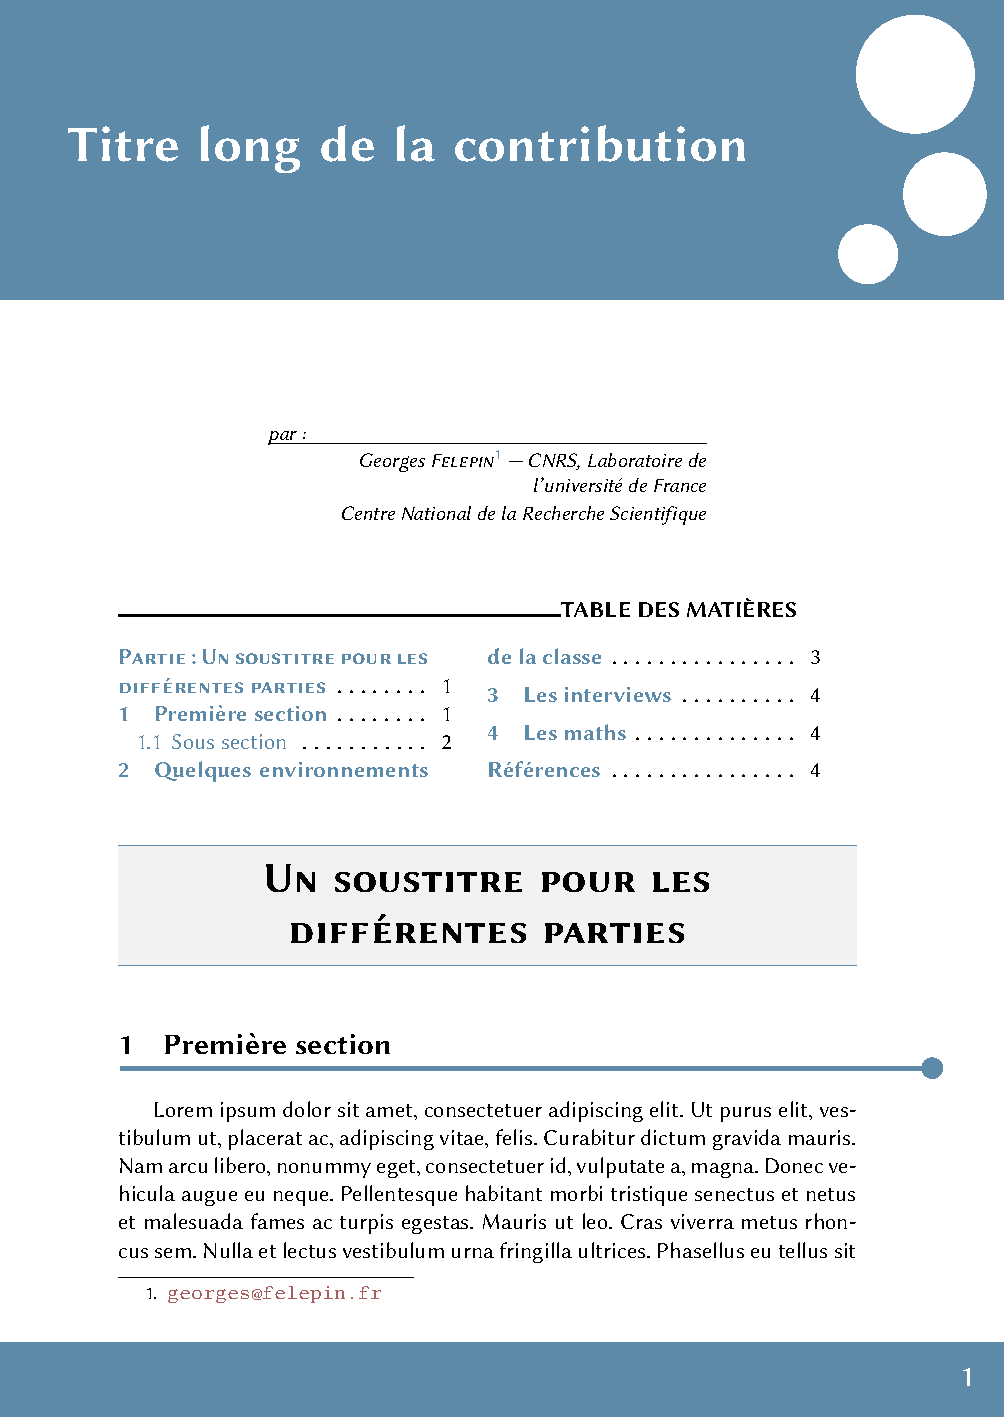
\includepdf[pages=-]{examples/modeleauteur/modele}

\subsection{La couverture}


\includepdf[pages=-]{examples/couverture/couvertureModele}

\printbibliography




\end{document}

%%% Local Variables:
%%% flyspell-mode: 1
%%% ispell-local-dictionary: "french"
%%% TeX-engine: luatex
%%% End:
